\documentclass[border=5pt]{standalone}
\usepackage[T1]{fontenc}
\usepackage{amsmath,amssymb}
\usepackage{tikz}
\usetikzlibrary{shapes.geometric, arrows.meta, positioning, calc, fit, backgrounds}

\definecolor{inputbg}{HTML}{EAEFF5}
\definecolor{procbg}{HTML}{D6E6F5}
\definecolor{decbg}{HTML}{FFF3D0}
\definecolor{projbg}{HTML}{DCEDC8}
\definecolor{outbg}{HTML}{C8E6C9}
\definecolor{skipbg}{HTML}{FFE0B2}
\definecolor{mainedge}{HTML}{333333}
\definecolor{dashedge}{HTML}{5A5A5A}
\definecolor{scpimlp}{HTML}{3F51B5}
\definecolor{feedbk}{HTML}{2E7D32}

\begin{document}
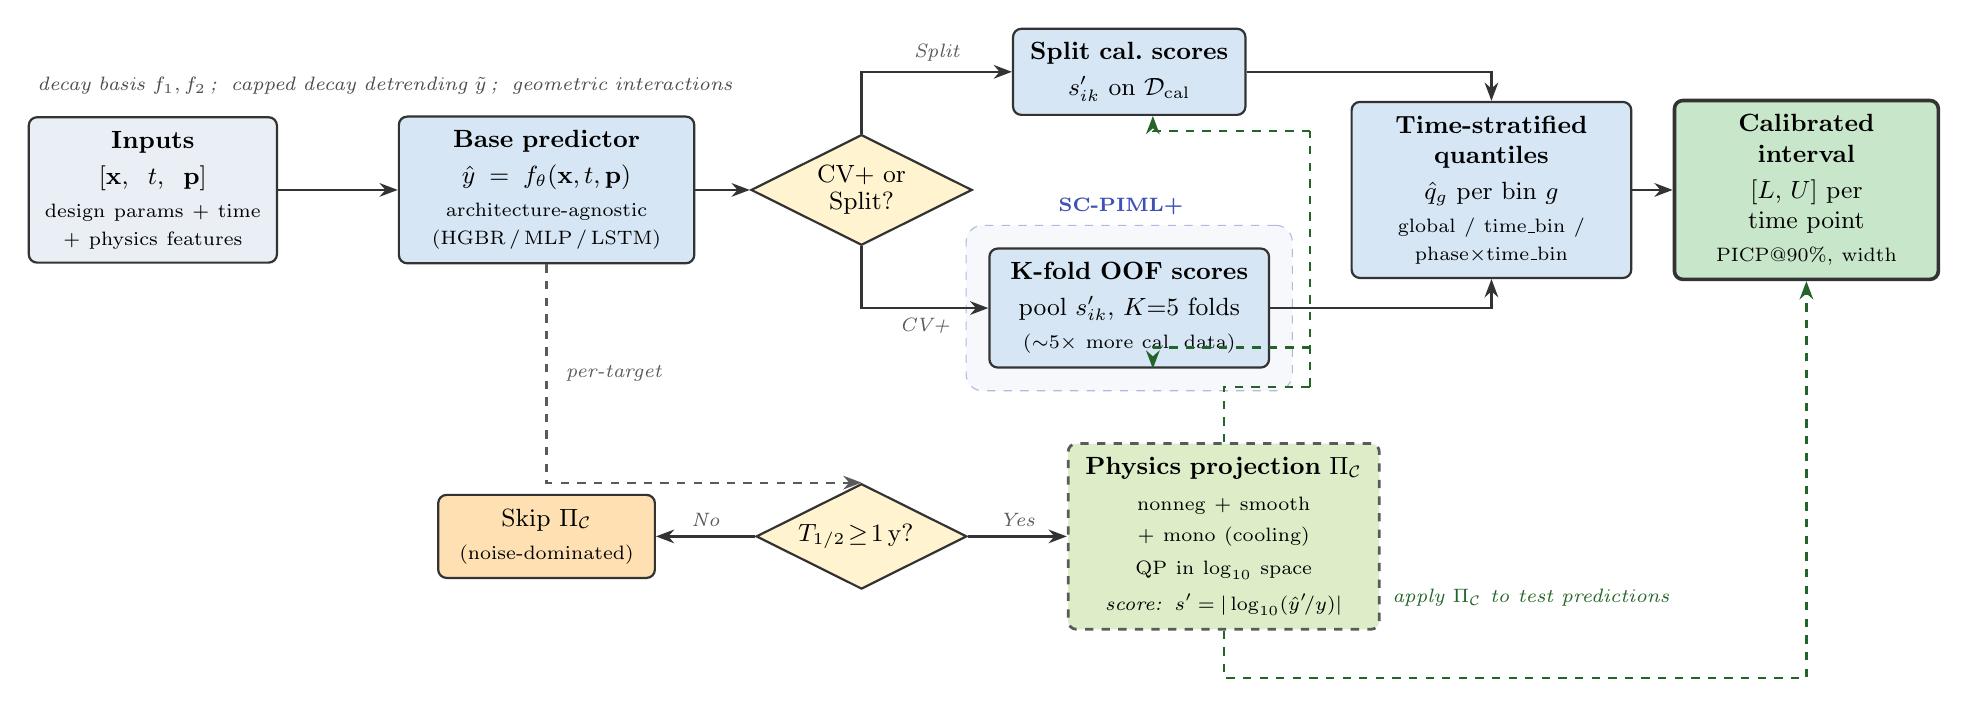
\begin{tikzpicture}[
    >=Stealth,
    every node/.style={font=\small},
    box/.style={
        rectangle, rounded corners=3pt, draw=mainedge, thick,
        minimum height=1.0cm, align=center, inner sep=5pt
    },
    mydiamond/.style={
        diamond, draw=mainedge, thick, aspect=2.0,
        inner sep=2pt, align=center, font=\small
    },
    elabel/.style={font=\scriptsize\itshape, text=dashedge},
    mainline/.style={->, thick, color=mainedge},
    dashline/.style={->, thick, dashed, color=dashedge},
    feedline/.style={->, thick, dashed, color=feedbk!80!black},
    note/.style={font=\scriptsize, text=gray!60!black},
]

%% ============ ROW 1: MAIN PIPELINE ============
%%
%% Layout budget (x-coordinates):
%%   inputs:  0        (w=2.8cm → ±1.4)   edges: [-1.4, 1.4]
%%   pred:    5.0      (w=3.4cm → ±1.7)   edges: [ 3.3, 6.7]
%%   cvdec:   9.0      diamond ~1.2 wide   edges: [ 7.8,10.2]
%%   split:  12.4      (w=2.6cm → ±1.3)   edges: [11.1,13.7]  +inner=0.18 → 13.88
%%   cvplus: 12.4      (w=3.2cm → ±1.6)   edges: [10.8,14.0]  +inner=0.18 → 14.18
%%   SC-PIML+ highlight: +8pt=0.28 → right edge ≈ 14.46
%%   FEEDBACK CORRIDOR: x = 14.7  (safely past all score boxes + highlight)
%%   quant:  17.0      (w=3.2cm → ±1.6)   edges: [15.4,18.6]
%%   output: 21.0      (w=3.0cm → ±1.5)   edges: [19.5,22.5]
%%

\node[box, fill=inputbg, text width=2.8cm] (inputs) at (0,0) {
    \textbf{Inputs}\\[2pt]
    $[\mathbf{x},\; t,\; \mathbf{p}]$\\[1pt]
    {\scriptsize design params + time}\\[-1pt]
    {\scriptsize + physics features}
};

\node[box, fill=procbg, text width=3.4cm] (pred) at (5.0,0) {
    \textbf{Base predictor}\\[2pt]
    $\hat{y} = f_\theta(\mathbf{x}, t, \mathbf{p})$\\[1pt]
    {\scriptsize architecture-agnostic}\\[-1pt]
    {\scriptsize (HGBR\,/\,MLP\,/\,LSTM)}
};

\node[mydiamond, fill=decbg] (cvdec) at (9.0,0) {
    CV+ or\\[-1pt]Split?
};

\node[box, fill=procbg, text width=2.6cm] (split) at (12.4, 1.5) {
    \textbf{Split cal.\ scores}\\[2pt]
    $s'_{ik}$ on $\mathcal{D}_\text{cal}$
};

\node[box, fill=procbg, text width=3.2cm] (cvplus) at (12.4, -1.5) {
    \textbf{K-fold OOF scores}\\[2pt]
    pool $s'_{ik}$, $K{=}5$ folds\\[1pt]
    {\scriptsize (${\sim}5{\times}$ more cal.\ data)}
};

\node[box, fill=procbg, text width=3.2cm] (quant) at (17.0, 0) {
    \textbf{Time-stratified}\\
    \textbf{quantiles}\\[2pt]
    $\hat{q}_g$ per bin $g$\\[1pt]
    {\scriptsize global / time\_bin /}\\[-1pt]
    {\scriptsize phase${\times}$time\_bin}
};

\node[box, fill=outbg, text width=3.0cm, line width=1.3pt] (output) at (21.0, 0) {
    \textbf{Calibrated interval}\\[2pt]
    $[L,\, U]$ per time point\\[1pt]
    {\scriptsize PICP@90\%, width}
};

%% ============ ROW 2: PROJECTION BRANCH ============

\node[mydiamond, fill=decbg] (hldec) at (9.0, -4.4) {
    $T_{1/2} \!\geq\! 1$\,y?
};

\node[box, fill=projbg, draw=dashedge, dashed, line width=1pt, text width=3.6cm] (proj) at (13.6, -4.4) {
    \textbf{Physics projection} $\Pi_{\mathcal{C}}$\\[2pt]
    {\scriptsize nonneg + smooth + mono (cooling)}\\[1pt]
    {\scriptsize QP in $\log_{10}$ space}\\[2pt]
    {\scriptsize\itshape score: $s'\!=\!|\log_{10}(\hat{y}'\!/y)|$}
};

\node[box, fill=skipbg, text width=2.4cm] (skip) at (5.0, -4.4) {
    Skip $\Pi_{\mathcal{C}}$\\[1pt]
    {\scriptsize (noise-dominated)}
};

%% ============ MAIN FLOW EDGES ============
\draw[mainline] (inputs) -- (pred);
\draw[mainline] (pred) -- (cvdec);
\draw[mainline] (cvdec.north) |- node[elabel, pos=0.75, above] {Split} (split.west);
\draw[mainline] (cvdec.south) |- node[elabel, pos=0.75, below] {CV+} (cvplus.west);
\draw[mainline] (split.east) -| (quant.north);
\draw[mainline] (cvplus.east) -| (quant.south);
\draw[mainline] (quant) -- (output);

%% ============ PROJECTION BRANCH EDGES ============
% predictor -> half-life check: vertical dashed line
\draw[dashline] (pred.south) -- (pred.south |- hldec.north) -- (hldec.north);
% "per-target" label: placed to the RIGHT of the vertical line, midway
\node[elabel, anchor=west] at ($(pred.south)!0.5!(pred.south |- hldec.north) + (0.12, 0)$) {per-target};

% half-life decisions
\draw[mainline] (hldec.east) -- node[elabel, above] {Yes} (proj.west);
\draw[mainline] (hldec.west) -- node[elabel, above] {No} (skip.east);

%% ============ FEEDBACK: PROJECTION -> SCORES ============
%%
%% Corridor at x=14.7, right of SC-PIML+ highlight edge (~14.46),
%% left of quantiles left edge (~15.4).
%% Route: proj.north ↑ y=-2.5 → right to corridor → up to y=0.75
%%

\pgfmathsetmacro{\fbx}{14.7}

% projection → corridor: L-shape (up, then right)
\draw[feedline, -] (proj.north) -- (13.6, -2.5) -- (\fbx, -2.5);

% corridor vertical: up from junction to split branch level
\draw[feedline, -] (\fbx, -2.5) -- (\fbx, 0.75);

% branch LEFT to split.south (+0.3 offset from center)
\draw[feedline] (\fbx, 0.75) -| ($(split.south) + (0.3, 0)$);

% branch LEFT to cvplus.south (+0.3 offset)
\draw[feedline] (\fbx, -2.0) -| ($(cvplus.south) + (0.3, 0)$);

%% ============ PROJECTION -> OUTPUT (apply to test) ============
%%
%% Route along the bottom of the figure to avoid crossing anything:
%% proj east -> horizontal at y=-5.2 -> right to x=21 -> up to output.south
%%
\draw[feedline] (proj.south) -- ++(0, -0.6) -| (output.south);

% Label on the horizontal bottom segment (fixed position, not pos=)
\node[elabel, text=feedbk!80!black, anchor=north]
    at (17.5, -4.95) {apply $\Pi_{\mathcal{C}}$ to test predictions};

%% ============ ANNOTATIONS ============
\node[note, anchor=south west, text width=10cm] at ($(inputs.north west) + (0, 0.15)$) {
    \textit{decay basis $f_1, f_2$\,;\; capped decay detrending $\tilde{y}$\,;\; geometric interactions}
};

%% SC-PIML+ highlight around CV+ box
\begin{scope}[on background layer]
    \node[draw=scpimlp!40, fill=scpimlp!4, rounded corners=6pt, dashed,
          fit=(cvplus), inner sep=8pt,
          label={[font=\scriptsize\bfseries, text=scpimlp, xshift=-3pt]above:SC-PIML+}] {};
\end{scope}

\end{tikzpicture}
\end{document}
